\documentclass[12pt]{article}

\usepackage{amsmath}
\usepackage{amssymb}

\usepackage{graphicx}
\usepackage{caption}
\usepackage{subcaption}

\usepackage{algorithm}% http://ctan.org/pkg/algorithms
\usepackage{algpseudocode}% http://ctan.org/pkg/algorithmicx
\usepackage{framed} % or, "mdframed"
\usepackage[framed]{ntheorem}
\usepackage{listings}
\usepackage{color}
\usepackage[usenames,dvipsnames,svgnames,table]{xcolor}

\newframedtheorem{frm-thm}{Lemma}

\usepackage[scale=1.0, left=1.0cm, right=1.0cm, top=1.865cm, bottom=0.865cm]{geometry}
\DeclareMathOperator*{\argmin}{arg\,min}

\definecolor{dkgreen}{rgb}{0,0.6,0}
\definecolor{dred}{rgb}{0.545,0,0}
\definecolor{dblue}{rgb}{0,0,0.545}
\definecolor{lgrey}{rgb}{0.9,0.9,0.9}
\definecolor{gray}{rgb}{0.4,0.4,0.4}
\definecolor{darkblue}{rgb}{0.0,0.0,0.6}
\lstset{
      backgroundcolor=\color{lgrey},
      basicstyle=\footnotesize \ttfamily \color{black} \bfseries,
      breakatwhitespace=false,
      breaklines=true,
      captionpos=b,
      commentstyle=\color{dkgreen},
      deletekeywords={...},
      escapeinside={\%*}{*)},
            frame=single,
      keywordstyle=\color{purple},
      morekeywords={BRIEFDescriptorConfig,string,TiXmlNode,DetectorDescriptorConfigContainer,istringstream,cerr,exit},
      identifierstyle=\color{black},
      stringstyle=\color{blue},
      language=C,
      numbers=right,
      numbersep=5pt,
      numberstyle=\tiny\color{black},
      rulecolor=\color{black},
      showspaces=false,
      showstringspaces=false,
      showtabs=false,
      stepnumber=1,
      tabsize=5,
      title=\lstname,
    }


\pagestyle{myheadings}
\markright{CSE 260, Assignment 2 \hfill Andrew Conegliano, Matthias Springer\hfill}

\begin{document}

\title{Double-Precision Matrix Multiply on CUDA  \\ \vspace{2 mm} {\large Parallel Computation (CSE 260), Assignment 2}}
\date{February 13, 2014}
\author{Andrew Conegliano (A53053325) \and Matthias Springer (A99500782) \and GID G-338-665}
\maketitle

\subsection*{Assumptions}
\begin{itemize}
        \item All matrices are square matrices and have a size of $256 \times 256$, $512 \times 512$, $1024 \times 1024$, or $2048 \times 2048$.
        \item All matrices consist of double-precision floating point values (64-bit doubles).
        \item Parameters (grid/block size) and matrix size are chosen in such a way that no fringe cases emerge.
\end{itemize}

\subsection*{Notation}
%\end{tabular}
In this work, we use the following notation and variable names.
\begin{itemize}
        \item $n$ is the size of one dimension of the matrices involved. I.e., every matrix has $n^2$ values.
        \item When referring to matrices, $A$ and $B$ denote the source matrices and $C$ denotes the target matrix, i.e. $C \leftarrow A * B$.
        \item $i_{B,x}$ and $i_{B,y}$ are the block index in x or y dimension, i.e. \lstinline{blockIdx.x/y}.
        \item $\mathit{dim}_{B,x}$ and $\mathit{dim}_{B,y}$ are the block dimension in x or y dimension, i.e. \lstinline{blockDim.x/y}.
        \item $i_{T,x}$ and $i_{T,y}$ are the thread index in x or y dimension, i.e. \lstinline{threadIndex.x/y}.
        \item $\mathit{dim}_{G,x}$ and $\mathit{dim}_{G,y}$ are the grid dimension in x or y dimension, i.e. \lstinline{gridDim.x/y}.
\end{itemize}

\section{Runtime Environment}
We optimized our implementation for a specific runtime environment. All benchmarks and performance results are based on the following hardware and software.

\subsection{Hardware (Dirac)}
\begin{itemize}
        \item 2 Nahalem Quad Core CPUs
        \item 24 GB DDR3 RAM
        \item 1 Tesla C2050 (Fermi) GPU
        \begin{itemize}
                \item 14 vector units $\times$ 32 cores = 448 total cores \@ 1.15 GHz
                \item 3 GB DDR5 RAM, 2.625 GB usable due to ECC
                \item L2 cache size: 786432 bytes
                \item Total constant memory: 65536 bytes
                \item Total shared memory per block: 49152 bytes
                \item Total number of registers per block: 32768
                \item Maximum number of threads per block: 1024
                \item Maximum block dimension: 1024 $\times$ 1024 $\times$ 64
                \item Maximum grid dimension: 65535 $\times$ 65535 $\times$ 65535
                \item Warp size: 32
                \item Double precision performance peak: 515 Gflops
        \end{itemize}
        \end{itemize}

\subsection{Software}
\begin{itemize}
	\item GNU/Linux, kernel version \texttt{2.6.32-358.14.1.el6.nersc9.x86\_64}
    \item CUDA 5.5
\end{itemize}

\section{Basic Algorithm}
%TODO: calculate occupancy
The basic algorithm uses a constant block size and grid dimension of $\mathit{dim}_{G,x} = \lceil \frac{n}{\mathit{dim}_{B,x}} \rceil$ and $\mathit{dim}_{G,y} = \lceil \frac{n}{\mathit{dim}_{B,y}} \rceil$. This ensures that enough threads are spawned, such that every value of $C$ is computed in a separate thread ($n^2$ threads).

\begin{figure}[H]
\begin{lstlisting}[mathescape]
c = 0

for k = 0 .. N - 1
	a = A[$i_{B,x}$ * $\mathit{dim}_{B,x} + i_{T,x}$ * N + k]
	b = B[k * N + $i_{B,y}$ * $\mathit{dim}_{B,y} + i_{T,y}$]
	c += a * b

C[($i_{B,x}$ * $\mathit{dim}_{B,x} + i_{T,x}$) * N + $i_{B,y}$ * $\mathit{dim}_{B,y} + i_{T,y}$] = c
\end{lstlisting}
\caption{Naive matrix multiplication algorithm kernel.}
\label{fig:naive_mul}
\end{figure}

\paragraph{Feasible parameter space}
The basic algorithm has two parameters that we can change: $\mathit{dim}_{B,x}$ and $\mathit{dim}_{B,y}$. A block cannot contain more than $1024$ threads, therefore $\mathit{dim}_{B,x} \times \mathit{dim}_{B,y} \leq 1024$. Furthermore, $\mathit{dim}_{B,x}, \mathit{dim}_{B,x} < 1024$, because that it maximum block dimension.

\paragraph{Performance Evaluation}
Figure~\ref{fig:basic_performance} shows the performance of the basic algorithm at different block sizes (powers of $2$) for $n=256$, $n=512$, $n=1024$, and $n=2048$. For $n=2048$, we ran the algorithm 5 times and took the average value. For all other matrix sizes, we ran the algorithm 10 times. The white cells in the figure denote invalid combinations of block sizes, i.e. $\mathit{dim}_{B,x} \times \mathit{dim}_{B,y} > 1024$.

\begin{figure}[H]
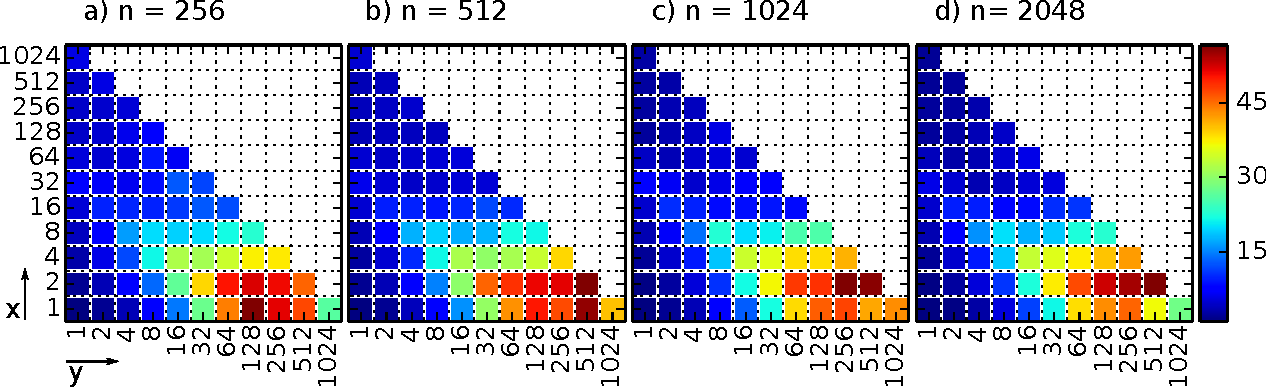
\includegraphics[width=\textwidth]{original_heat.pdf}
\caption{Basic Matrix Multiplication Algorithm at different block sizes.}
\label{fig:basic_performance}
\end{figure}

\noindent We reached the following peak performance at certain block sizes.
\begin{itemize}
	\item $n=256$: 58.3 GFlops at block size $1 \times 128$
    \item $n=512$: 54.3 GFlops at block size $2 \times 512$ \\
          $n=512$: 53.4 GFlops at block size $1 \times 512$
    \item $n=1024$: 56.6 GFlops at block size $2 \times 256$ \\
          $n=1024$: 56.1 GFlops at block size $2 \times 512$
   	\item $n=2048$: 56.5 GFlops at block size $2 \times 512$
\end{itemize}

\section{Optimizations}
In this section, we present optimizations, that increased the performance of the algorithm beyond 100 GFlops.

\subsection{Shared Memory}
The first optimization we attempted was to increase the use of shared memory. Shared memory is much faster, at 144 GB/s, than global memory. The basic algorithm makes each thread act independently. By applying the block algorithm, where small blocks of A and B are computed on instead of rows of A and B, we force the use of shared memory, and make threads cooperate. Each thread now loads in a single value of the needed rows/columns of the block into shared memory, then reads from shared memory the values needed for matrix multiplication. This optimization localizes memory accesses to only occur in shared memory, instead of global. 

Let us assume that we use a block size of $\mathit{dim}_B \times \mathit{dim}_B$, i.e. we use square block sizes. Then, every element of $A$ and $B$ that is loaded into shared memory, is reused $\mathit{dim}_B$ times, because every element in $A$ or $B$ is used or one row or column of a block in $C$. Shared memory can, therefore, reduce the global memory traffic.

\begin{figure}[H]
\begin{lstlisting}[mathescape]
(shared) a[$\mathit{dim}_{B,x}$][$\mathit{dim}_{B,y}$], b[$\mathit{dim}_{B,x}$][$\mathit{dim}_{B,y}$]
c = 0

for k = 0 .. $\mathit{dim}_{G,y}$
	a[$i_{T,x}$][$i_{T,y}$] = A[($i_{B,x}$ * $\mathit{dim}_{B,x}$ + $i_{T,x}$) * N+k * $\mathit{dim}_{B,y}$ + $i_{T,y}$]
	b[$i_{T,y}$][$i_{T,x}$] = B[($i_{B,y}$ * $\mathit{dim}_{B,y}$ + $i_{T,y}$) + N * (k * $\mathit{dim}_{B,x}$ + $i_{T,x}$)]
    (synchronize)
    
	for kk = 0 .. $\mathit{dim}_{B,x}$
		c += a[kk][$i_{T,x}$] * b[kk][$i_{T,y}$]
    (synchronize)
    
C[($i_{B,x}$ * $\mathit{dim}_{B,x}$ + $i_{T,x}$)*N + ($i_{B,y}$ * $\mathit{dim}_{B,y}$ + $i_{T,y}$)] = c
\end{lstlisting}
\caption{Shared memory optimization.}
\label{fig:shared_mem}
\end{figure}

\noindent Unfortunately, using this optimization barely improved performance because on the Kepler architecture, global memory references are cached.

\subsubsection{Implementation Details}
Note, that in Figure~\ref{fig:shared_mem}, we need to synchronize all threads after we buffer a block of $A$ and $B$ and after we computed the multiplications, to ensure that the whole block is buffered when the multiplications start and to ensure that no data from the next block is already loaded while some threads still compute multiplications for the previous block.

\subsubsection{Parameter Tuning}
In this section, the tile size is the number of elements that are cached in the global memory. We show two possible optimizations that we did not implement because of the drawbacks presented in the subsections.

\paragraph{Non-square block sizes}
We considered the case where block sizes are not square and the tile size equals the block size. Without loss of generality, let $x$ be the bigger dimension, i.e. $\mathit{dim}_{B,x} > \mathit{dim}_{B,y}$. Threads $(\mathit{dim}_{B,y} + 1, p), 0 \leq p < \mathit{dim}_{B,y}$ will read values from $A$ and put them into global memory. They will, however, not read the corresponding values\footnote{Coordinates are relative to the current block.} $(q, \mathit{dim}_{B,y} + 1), 0 \leq q < \mathit{dim}_{B,x}$, because these are not included in the current block. Since we need them for the multiplication, the only way to get them would be from global memory. Therefore, we should always choose square block sizes, if we want to take full advantage of shared memory.

\paragraph{Block size differing from tile size}
We considered the case where block sizes are square but bigger than the tile size. Since the block size equals the number of threads per block, there will either be threads that do not load any elements from $A$ or $B$, or data is loaded from $A$ and $B$ multiple times (redundantly).  This diminishes the effect of shared memory. Furthermore, elements will have to be loaded into the global memory multiple times. Therefore, if we run out of global memory, it is better to decrease the block size instead of adding another level of blocking inside blocks. 

It is, however, possible to run have multiple small tiles per block, effectively resulting in a second level of blocking inside CUDA blocks. This also allows us to use non-square CUDA block sizes. This optimization is discussed in a later subsection.

\subsubsection{Performance Evaluation}
\begin{figure}[H]
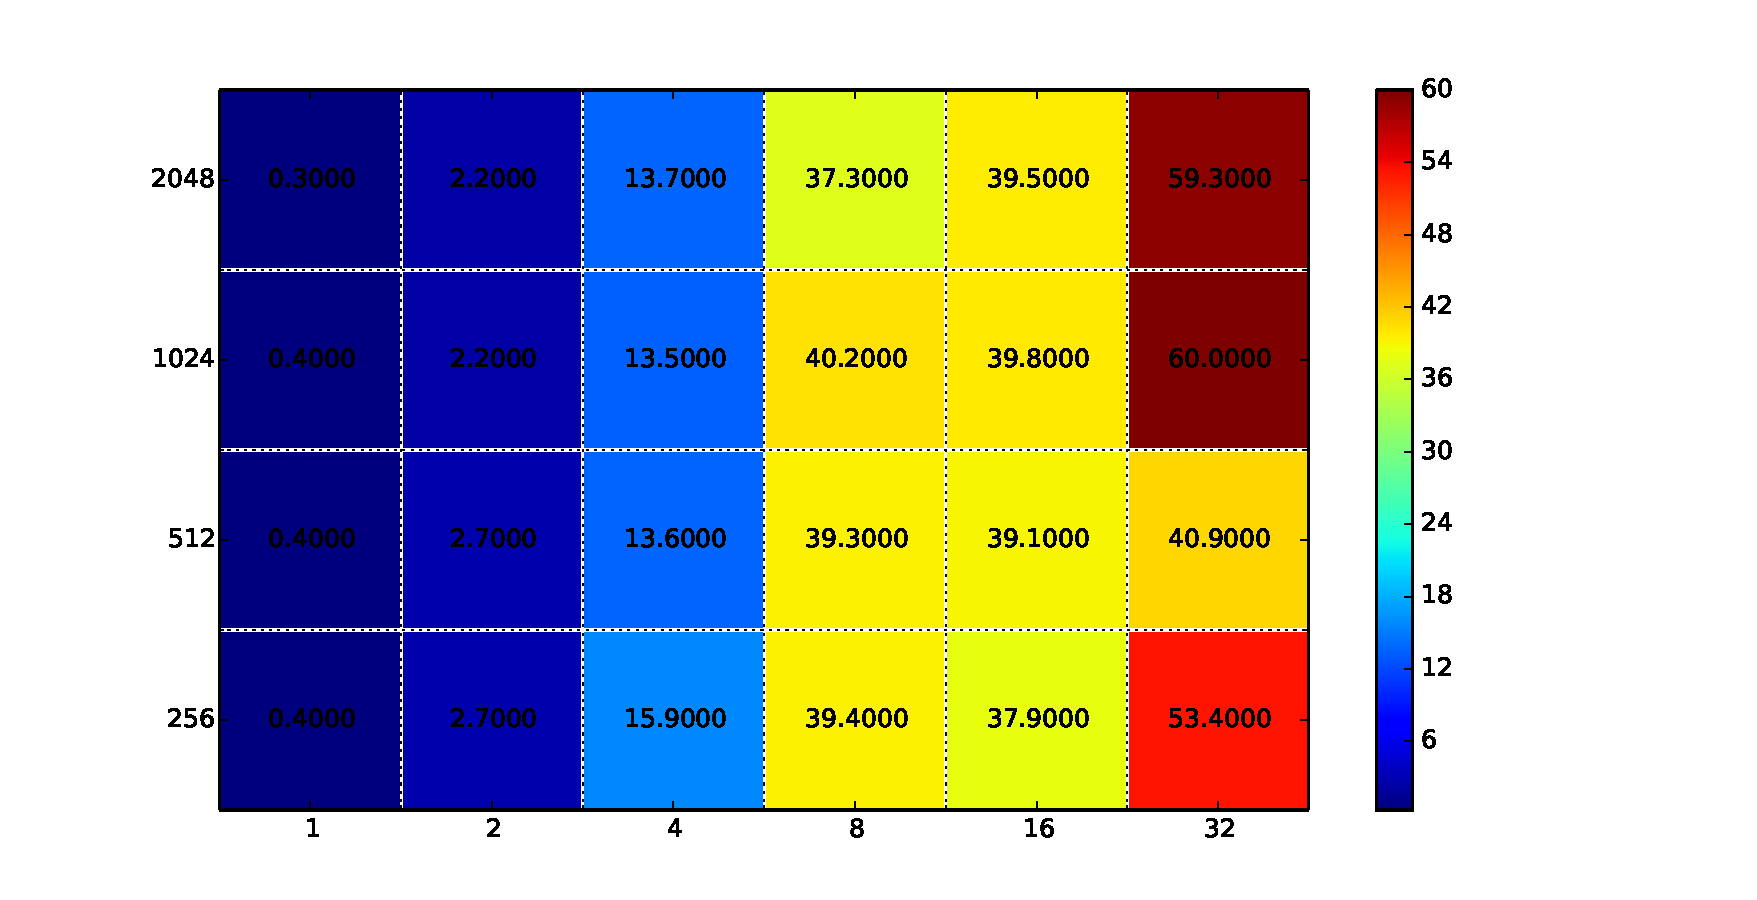
\includegraphics[width=\textwidth]{blocked_heat_scaled.pdf}
\caption{Matrix Multiplication Algorithm using shared memory.}
\label{fig:blocked_performance}
\end{figure}

\subsection{Memory Coalescing and Memory Banks}
In order for faster memory access, coalescing and memory block optimization was implemented. To coalesce global memory basically means to access it in rows sequentially and not columns. We made every thread accesses global memory in row-wise and consecutively in rows by modifying global memory indices. This in turn allows the DRAM on the GPU to consolidate memory requests into a single request, which results in peak bandwidth transfer rate. Also, global memory accesses need to be within a 128 byte segment, and do not need to be in sequential order. Cudamalloc guarantees memory to be aligned by 256 bytes minimum. This means in certain cases, warps will need 2 transactions in order to complete a read instead of 1. To prevent bank conflicts, threads need to access shared memory in columns or in offsets of $16(half warp)*32bits$. Every consecutive 32 bits of shared memory is allocated to different bank, max of 32 banks, and half warps are run at a time. Threads are organized by row sequentially, but access shared memory column wise. This allows each thread to access one memory bank, and because only one thread can access a memory bank at a time there are no conflicts.
\subsection{Implementation Details}
When accessing $A$ and storing it into shared memory, the $k * \mathit{dim}_{B,y}$ allows rows to be loaded and the $i_{T,x}$ are consecutive in value and in the same warp. Each thread accesses elements in the same row, and because all adjacent threads in warps access adjacent elements, the hardware will coalesce the access. The same logic is applied to the $B$ matrix. Memory banks are not conflicted because of the exception of all threads accessing the same 32-bit word, then its a broadcast.

\begin{figure}[H]
\begin{lstlisting}[mathescape]
(shared) a[$\mathit{dim}_{B,x}$][$\mathit{dim}_{B,y}$], b[$\mathit{dim}_{B,x}$][$\mathit{dim}_{B,y}$]
c = 0

for k = 0 .. $\mathit{dim}_{G,y}$
	a[$i_{T,x}$][$i_{T,y}$] = A[($i_{B,y}$ * $\mathit{dim}_{B,y}$ + $i_{T,y}$) * N+k * $\mathit{dim}_{B,y}$ + $i_{T,x}$]
	b[$i_{T,y}$][$i_{T,x}$] = B[($i_{B,x}$ * $\mathit{dim}_{B,x}$ + $i_{T,x}$) + N * (k * $\mathit{dim}_{B,x}$ + $i_{T,y}$)]
    (synchronize)
    
	for kk = 0 .. $\mathit{dim}_{B,x}$
		c += a[$i_{T,y}$][kk] * b[kk][$i_{T,x}$]
    (synchronize)
    
C[($i_{B,y}$ * $\mathit{dim}_{B,x}$ + $i_{T,y}$)*N + ($i_{B,y}$ * $\mathit{dim}_{B,y}$ + $i_{T,y}$)] = c
\end{lstlisting}
\caption{Coalesced memory optimization.}
\label{fig:coa_mem}
\end{figure}
\subsubsection{Performance Evaluation}
\begin{figure}[H]
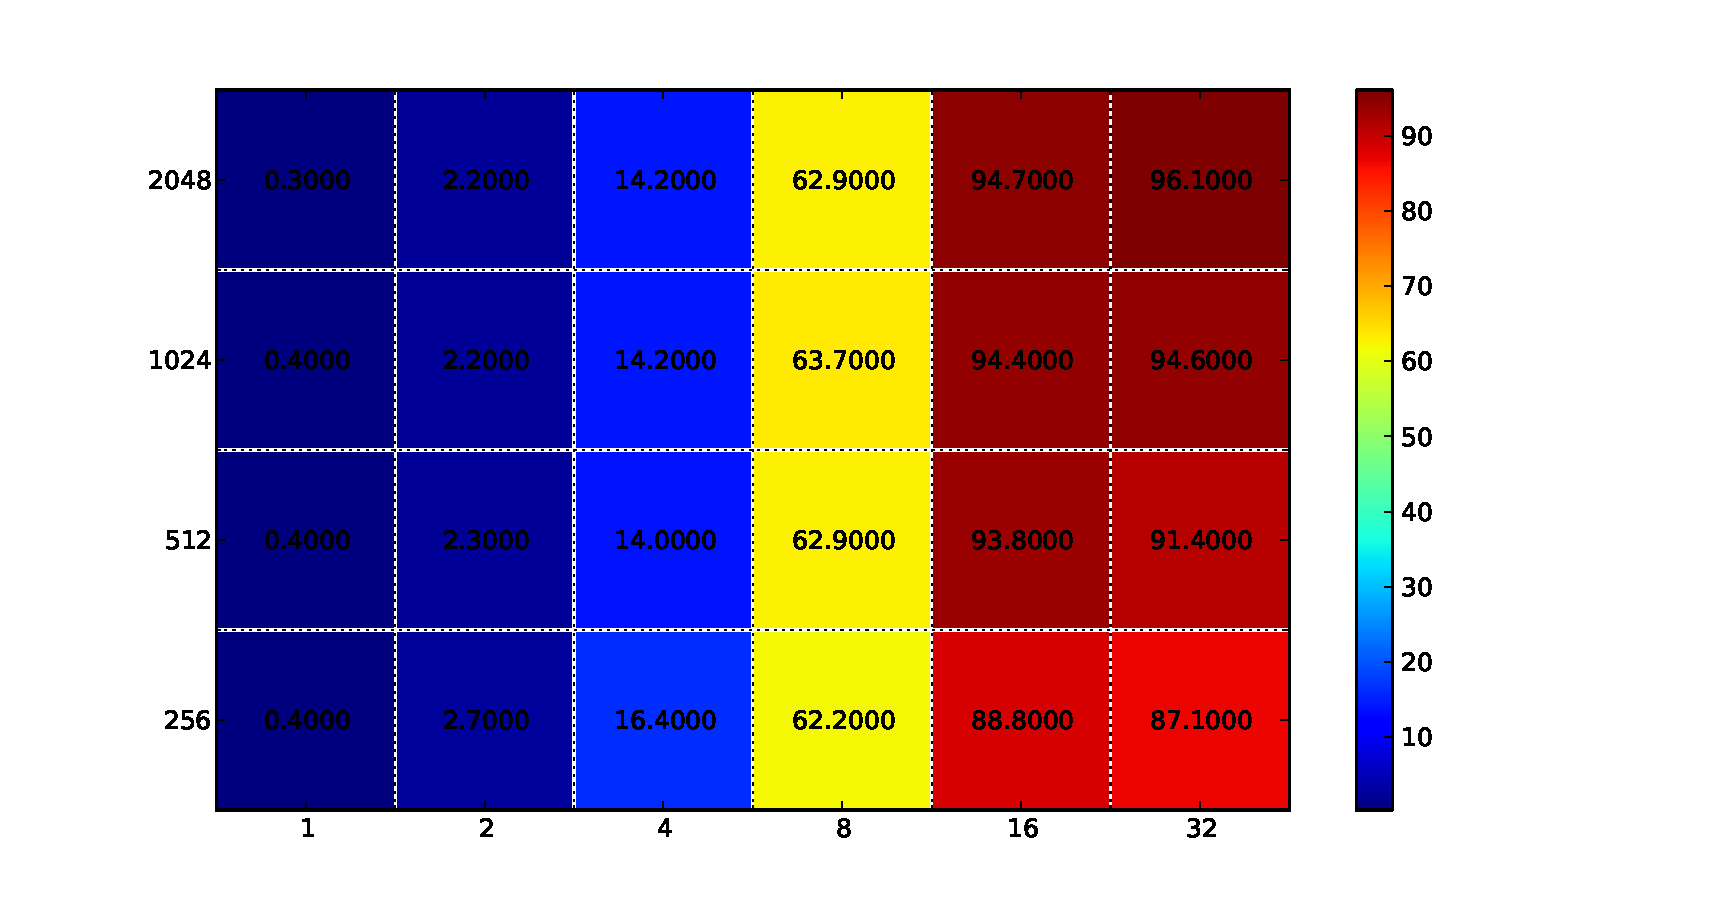
\includegraphics[width=\textwidth]{blocked_heat_coalesced_scaled.pdf}
\caption{Matrix Multiplication Algorithm using shared memory and coalescing.}
\label{fig:coa_performance}
\end{figure}

\subsection{Instruction Level Parallelism}
In order to hide memory latency, we chose to increase instruction level parallelism and sacrifice occupancy. The hardware in use needs to keep about 155KB of memory in flight, $~500CP(1100 nsec) * 144 GB/s$, which is met by the amount of threads used. Each thread now has an additional two memory stores and two multiply and add's (MAD), as well as an increase of 4x shared memory. This in turn increased the register use from 22 to 33. Registers are the only way to increase flops because they are the closest memory hierarchy to the hardware, hence the fastest.

\subsubsection{Implementation Details}
While keeping the block size constant, we reduced the grid dimension by a factor of 2 in both the $x$ and $y$ direction. Therefore, every thread stores 4 values of the original matrix into shared memory, does 4 MAD's, and computes 4 values of $C$, instead of just 1. A single thread computes the following values of C.

\begin{itemize}
	\item C[$i_{B,x} \times \mathit{dim}_{B,x} + i_{T,x}$][$i_{B,y} \times \mathit{dim}_{B,y} + t_{T,y}$]
    \item C[$(i_{B,x} + \mathit{dim}_{G,x}) \times \mathit{dim}_{B,x} + i_{T,x}$][$i_{B,y} \times \mathit{dim}_{B,y} + t_{T,y}$]
   	\item C[$i_{B,x} \times \mathit{dim}_{B,x} + i_{T,x}$][$(i_{B,y} + \mathit{dim}_{G,y}) \times \mathit{dim}_{B,y} + t_{T,y}$]
     \item C[$(i_{B,x} + \mathit{dim}_{G,x}) \times \mathit{dim}_{B,x} + i_{T,x}$][$(i_{B,y} + \mathit{dim}_{G,y}) \times \mathit{dim}_{B,y} + t_{T,y}$]
\end{itemize}

\begin{figure}[H]
        \centering
        \begin{subfigure}[b]{0.45\textwidth}
        		\centering
                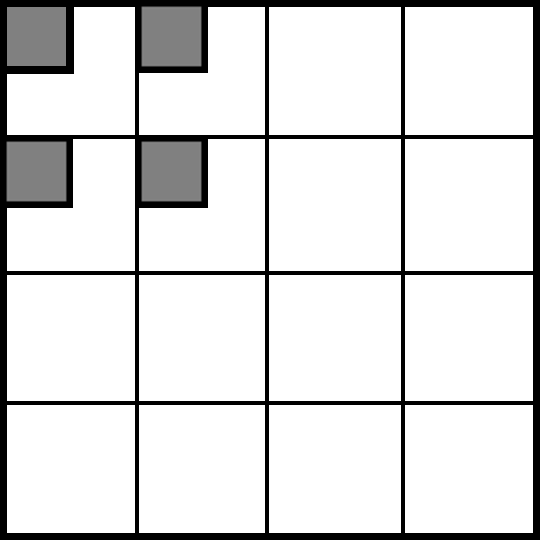
\includegraphics[width=0.5\textwidth]{blocks_blocked.pdf}
                \caption{Calculating elements of neighboring blocks.}
                \label{fig:block_neighboring}
        \end{subfigure}%
        ~ %add desired spacing between images, e. g. ~, \quad, \qquad etc.
          %(or a blank line to force the subfigure onto a new line)
        \begin{subfigure}[b]{0.45\textwidth}
        		\centering
                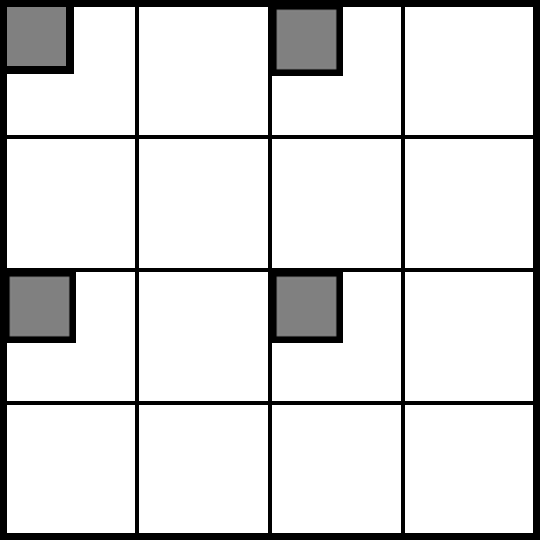
\includegraphics[width=0.5\textwidth]{blocks_distributed.pdf}
                \caption{Calculating elements of blocks that are far away.}
                \label{fig:block_far_away}
        \end{subfigure}
        \caption{Comparing access schemes of $C$ when decreasing grid dimension by 2 in both dimensions. Our kernel uses the scheme shown in Figure~\ref{fig:block_far_away}.}\label{fig:access_schemes}
\end{figure}

Figure~\ref{fig:access_schemes} shows two ways of distributing the extra computations that are done by one thread onto to matrix. In Figure~\ref{fig:block_neighboring}, every block computes the values that are contained in the original neighboring block\footnote{Keep in mind that the figure shows only one thread. The thin lines denote the original block boundaries.}. In Figure~\ref{fig:block_far_away}, every thread, and therefore every block, computes elements that are far way. The latter scheme proved to be more performant and is used in our final implementation.  When the computed elements are far away, it is less likely that threads access the same memory bank, resulting in a higher transfer rate from global memory to shared memory.

\subsubsection{Performance Evaluation}
\begin{figure}[H]
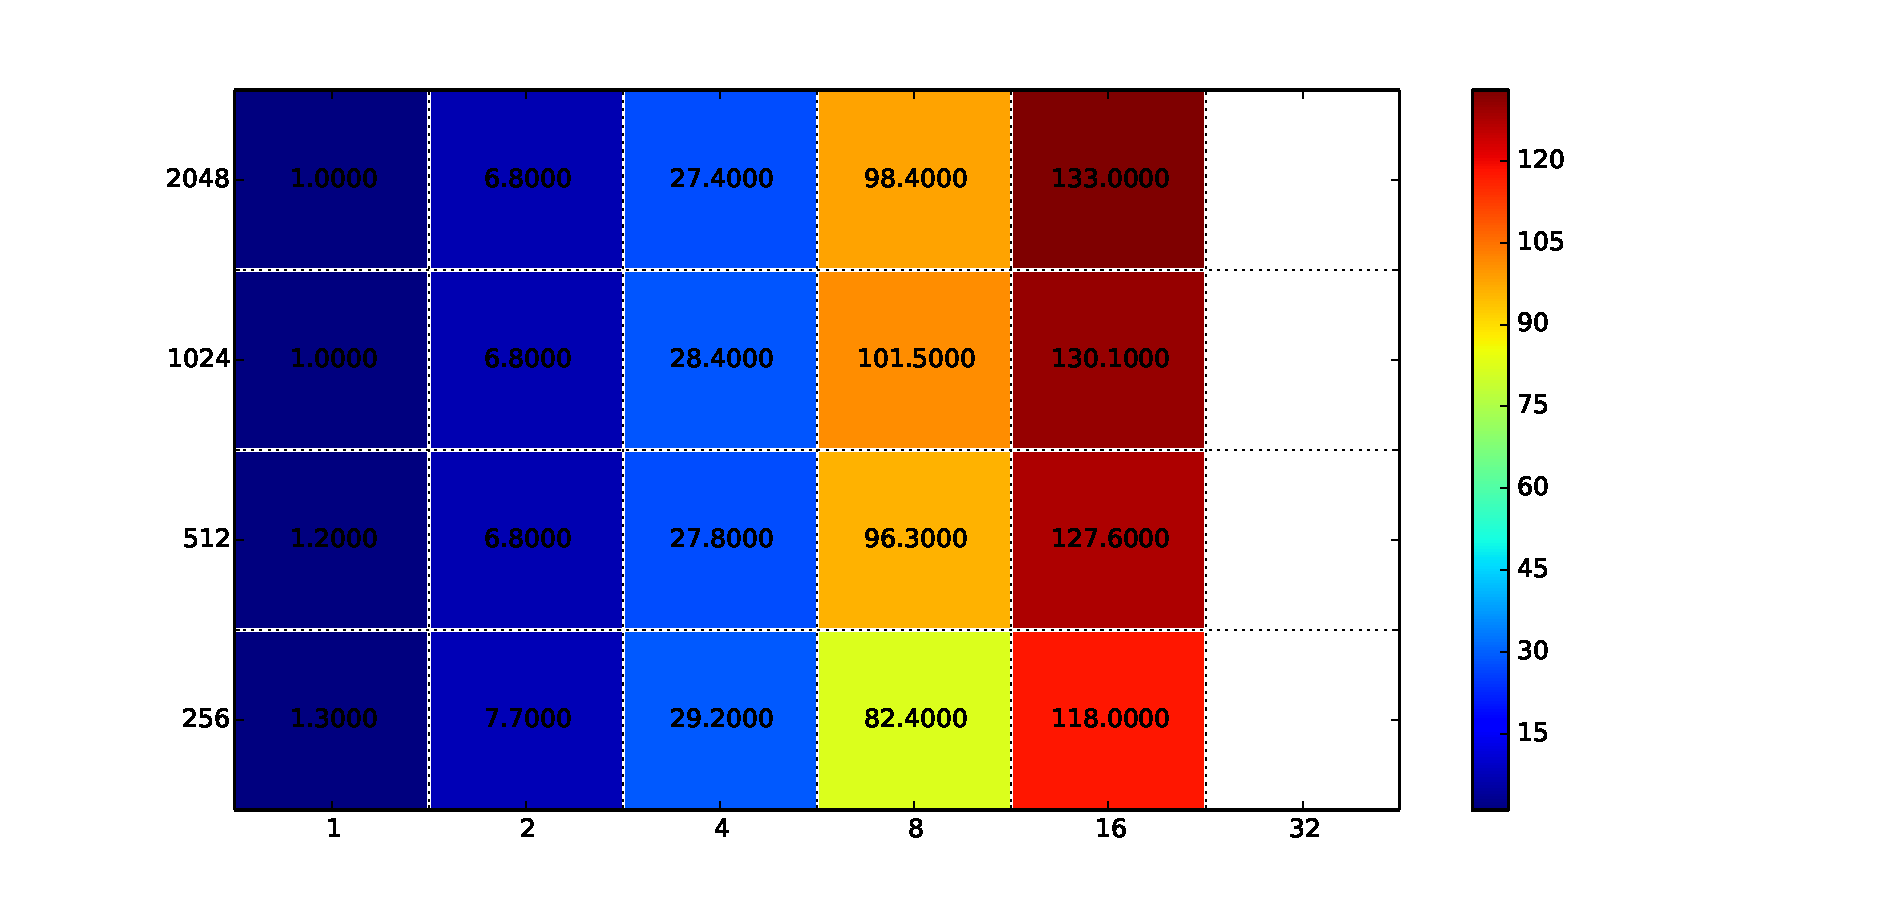
\includegraphics[width=\textwidth]{unrolled_a_b.pdf}
\caption{Matrix Multiplication Algorithm using shared memory, coalescing, and ILP.}
\label{fig:blocked_performance}
\end{figure}

Figure~\ref{fig:blocked_performance} shows the performance of the our final implementation with all optimizations except for second-level blocking. Note, that a block size of 32 is not feasible, because it exceeds the number of registers per block ($33 \times 32 \times 32 = 33792 > 32768$). Also, due to the unrolling, we use $\mathit{dim}_{B,x} \times \mathit{dim}_{B,y} \times 2$ doubles per matrix $A$ and $B$, resulting in $\mathit{dim}_{B,x} \times \mathit{dim}_{B,y} \times 32$ bytes, which is $32768$ bytes per block for $\mathit{dim}_{B,x} = \mathit{dim}_{B,y} = 32$. This does, however, not exceed the maximum shared memory per block.

\subsubsection{Increasing ILP}
We also tried to increase ILP further while maintaining square block sizes, by putting even more computations into one thread. This increases the shared memory usage. However, this optimization turned out to be slower. For example, by doing $8 \times 8 = 64$ computations per thread at a block size of $16 \times 16$, we utilized $63 \times 16 \times 16 = 16128$ registers per block (out of 32768) and $16 \times 16 \times 2 \times 8 \times 8 = 32786$ bytes shared memory (out of 49152), but it could not make up for the lost occupancy. The performance dropped to 12.5 GFlops at $n=1024$ and similar values for other matrix sizes.
%In theory, shared memory usage could be increased by a factor of $12$ at a block size of $16$

\subsection{Second-level Blocking}
In a previous subsection, we explained why the usage of shared memory restricts us to square block sizes. We can circumvent this restriction by adding a second level of blocking per CUDA block. Consider, for instance, that we have a block size of $8 \times 2$. When using only one level of blocking, we will eventually run into an \emph{index out of bounds} error, when we try to access the shared memory copy of $A$ or $B$ at the positions $(1,3), (1,4), \ldots$, because the algorithm expects a square matrix in the inner \texttt{kk} loop (see Figure~\ref{fig:coa_mem}).

Second-level blocking creates smaller blocks inside a CUDA block. In the $8 \times 2$ example, we create 4 inner blocks of size $2 \times 2$, i.e. the first 4 threads fill a shared memory block, the next 4 threads fill another shared memory block, and so on. These four inner blocks reside inside the same CUDA blocks, but the respective threads do not access shared data from other inner blocks.

\begin{figure}[H]
\centering
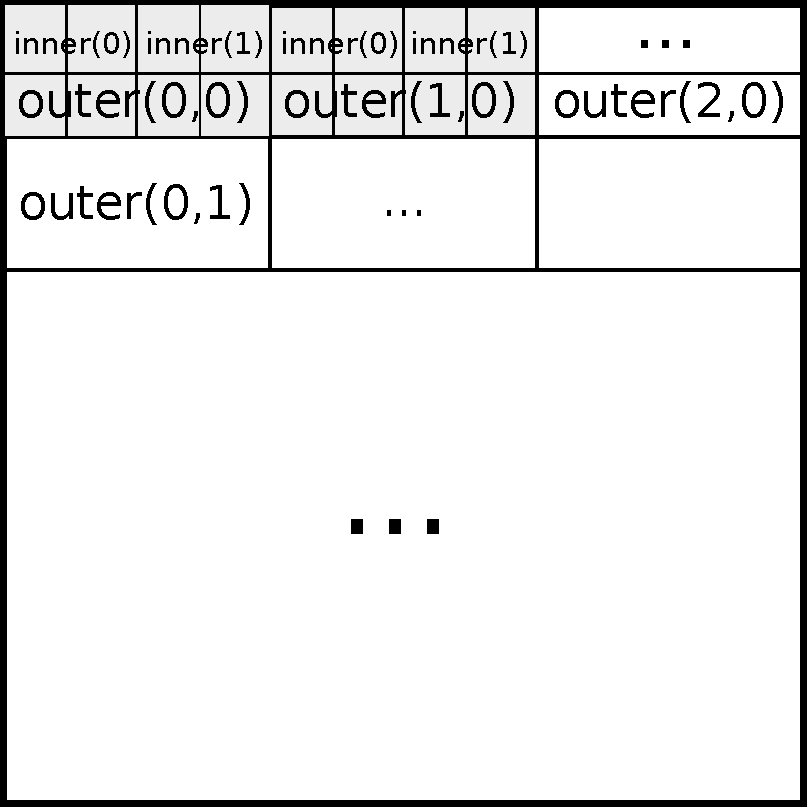
\includegraphics[width=0.25\textwidth]{inner_outer.pdf}
\caption{Second-level blocking: Creating inner blocks inside outer (CUDA) blocks.}
\label{fig:inner_outer}
\end{figure}

Figure~\ref{fig:inner_outer} shows an example for second-level blocking at a CUDA (outer) block size of $8 \times 4$. Every inner block has size $4 \times 4$ and is, therefore, square.

\subsubsection{Implementation Details}
We try to keep the number of inner blocks as small as possible. A smaller number of inner blocks results in bigger inner blocks, and a big block size results in more reuse of data, as explained in Section~3.1. 

Therefore, we divide a CUDA block of size $\mathit{dim}_{B,x} \times \mathit{dim}_{B,y}$ into inner blocks as follows. Let, without loss of generality, $\mathit{dim}_{B,x} > \mathit{dim}_{B,y}$\footnote{For $\mathit{dim}_{B,x} = \mathit{dim}_{B,y}$, we just create a single inner block.}. Then we have an inner grid dimension of $\frac{\mathit{dim}_{B,x}}{\mathit{dim}_{B,y}} \times 1$. Note, that since we assume that $\mathit{dim}_{B,x}$ and $\mathit{dim}_{B,y}$ divide $n$ evenly, $\mathit{dim}_{B,x}$ is always a multiple of $\mathit{dim}_{B,y}$ for matrix sizes of $256$, $512$, $1024$ and $2048$\footnote{These are the matrix sizes re ran benchmarks for.}. Every inner block has a size of $\mathit{dim}_{B,y} \times \mathit{dim}_{B,y}$.

\subsubsection{Performance Evaluation}
\begin{figure}[H]
\centering
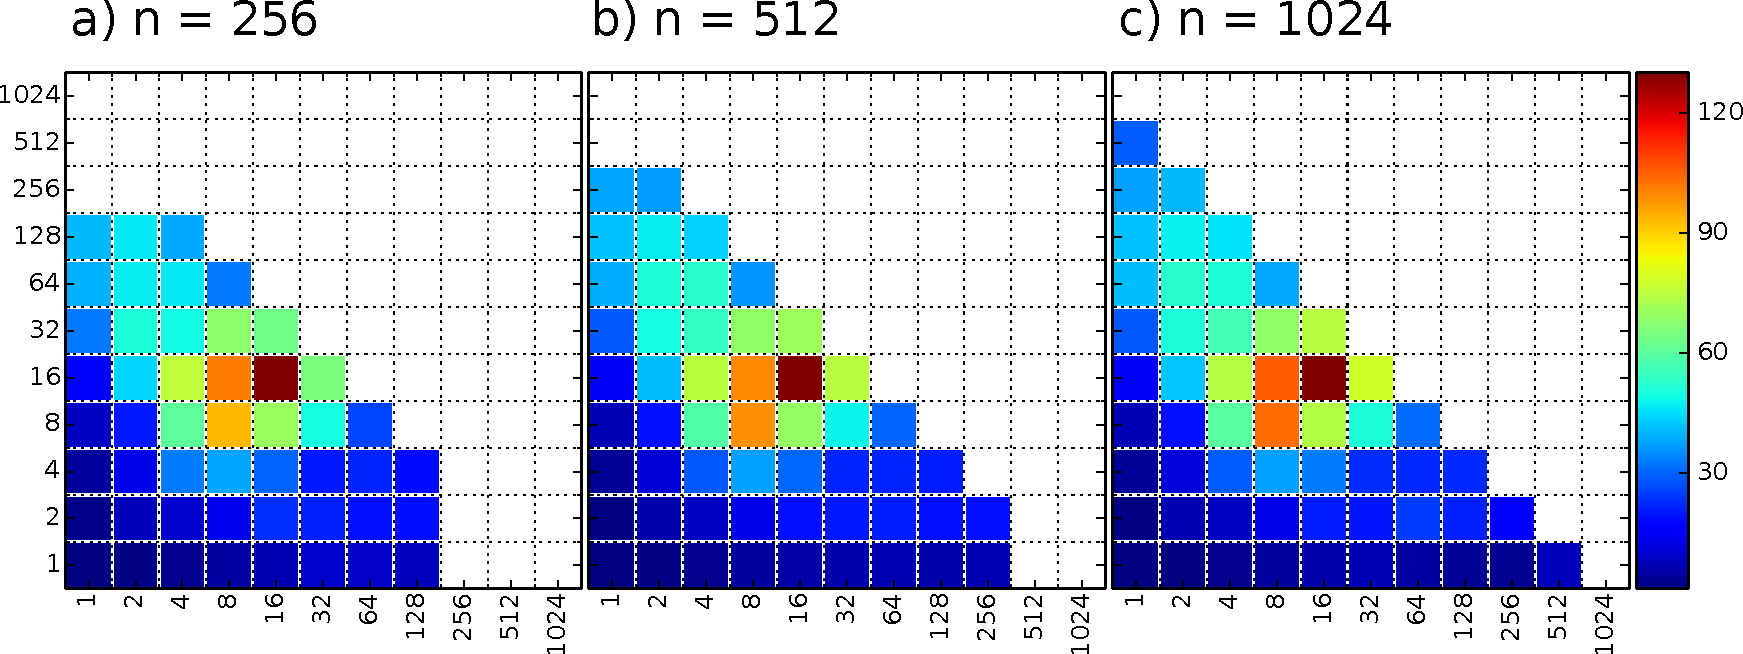
\includegraphics[width=\textwidth]{heat_final.pdf}
\caption{Performance of coalesced, shared-memory algorithm with ILP and second-level blocking at different block sizes.}
\label{fig:final_block_perf}
\end{figure}

Figure~\ref{fig:final_block_perf} shows the performance of our final algorithm at different block sizes. For a (CUDA) block size of $16 \times 16$, we reach the peak performance (same as in the previous subsection). In this case, we create only one inner block. This results in the maximum reuse of shared memory, because the inner block is as big as possible. For the next bigger CUDA block size (that devides $256$, $512$, or $1024$ evenly) of $32 \times 32$, we run out of registers, thus this configuration is not feasible.

Note, that for $n=256$, the configurations $1 \times 256$ and $256 \times 1$ are invalid. The same is the case for $n=512$ and $n=1024$. The reason is that our algorithm computes two values of $C$ at a time per thread, due to the ILP optimization presented in a previous subsection. Therefore, $n=256$ and $1 \times 256$ (and the other configurations mentioned) are not feasible, because they leave no space for ILP/unrolling in y direction.

\subsection{Further Considerations}
% There is no thread divergence
Our kernel has no fringe cases because we assume a matrix size evenly divisible by our block sizes. Our kernel also has no thread divergence, because all threads inside one block always follow the same instruction stream. There are no \texttt{if} statements that could cause the kernel to diverge.

\section{Host CPU computation}
Figure~\ref{fig:perf_host} shows the performance of the multi-threaded matrix multiplication algorithm that runs on the host CPUs at different matrix sizes and number of threads. For the matrix size, we chose multiples of $32$ between $512$ and $1504$, because we were told that we can reach the peak performance for matrix sizes close to $1024$. The results from the last assignment suggest that the peak performance is reached at multiples of $32$ (or other powers of 2).

\begin{figure}[H]
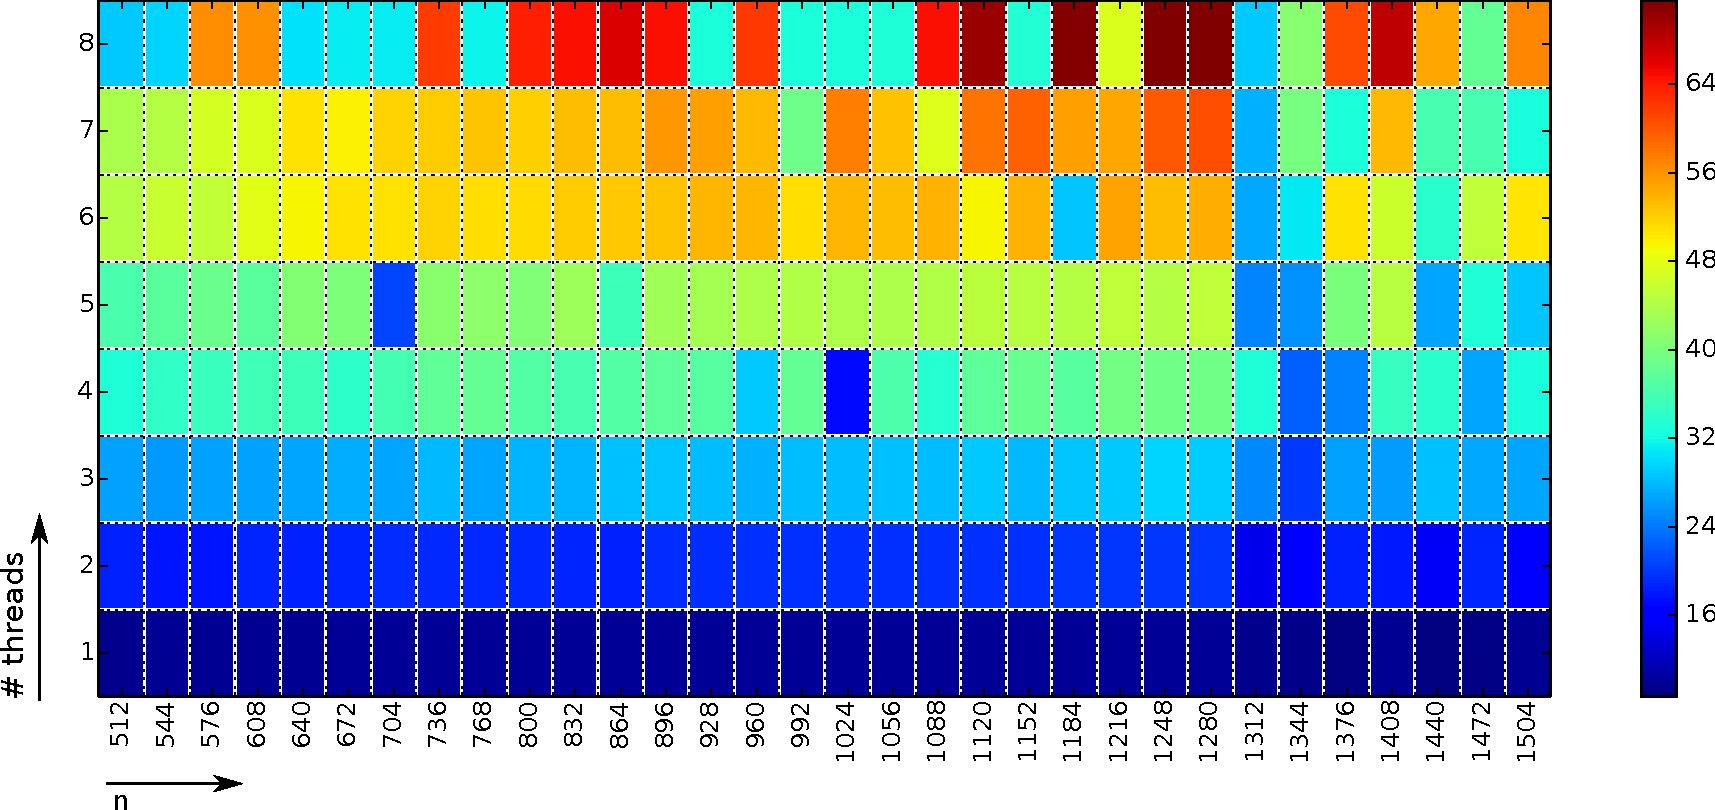
\includegraphics[width=\textwidth]{heat_host_cpu.pdf}
\caption{Host CPU multi-threaded performance}
\label{fig:perf_host}
\end{figure}

For the following parameters, we reached the peak performance. We ran the algorithm for every parameter setting 10 times and took the average value.
\begin{itemize}
	\item $n=1120$, 8 threads: 69.95 GFlops
    \item $n=1184$, 8 threads: 71.11 GFlops
    \item $n=1248$, 8 threads: 71.55 GFlops
    \item $n=1280$, 8 threads: 71.54 GFlops
\end{itemize}

\section{Performance Overview}
Figure~\ref{fig:overview} gives an overview of all optimizations and the performance the single-threaded host CPU computation\footnote{This is the performance of the unoptimized host verification code.}. The CUDA bars show the performance for the best parameters (block size).

\begin{figure}[H]
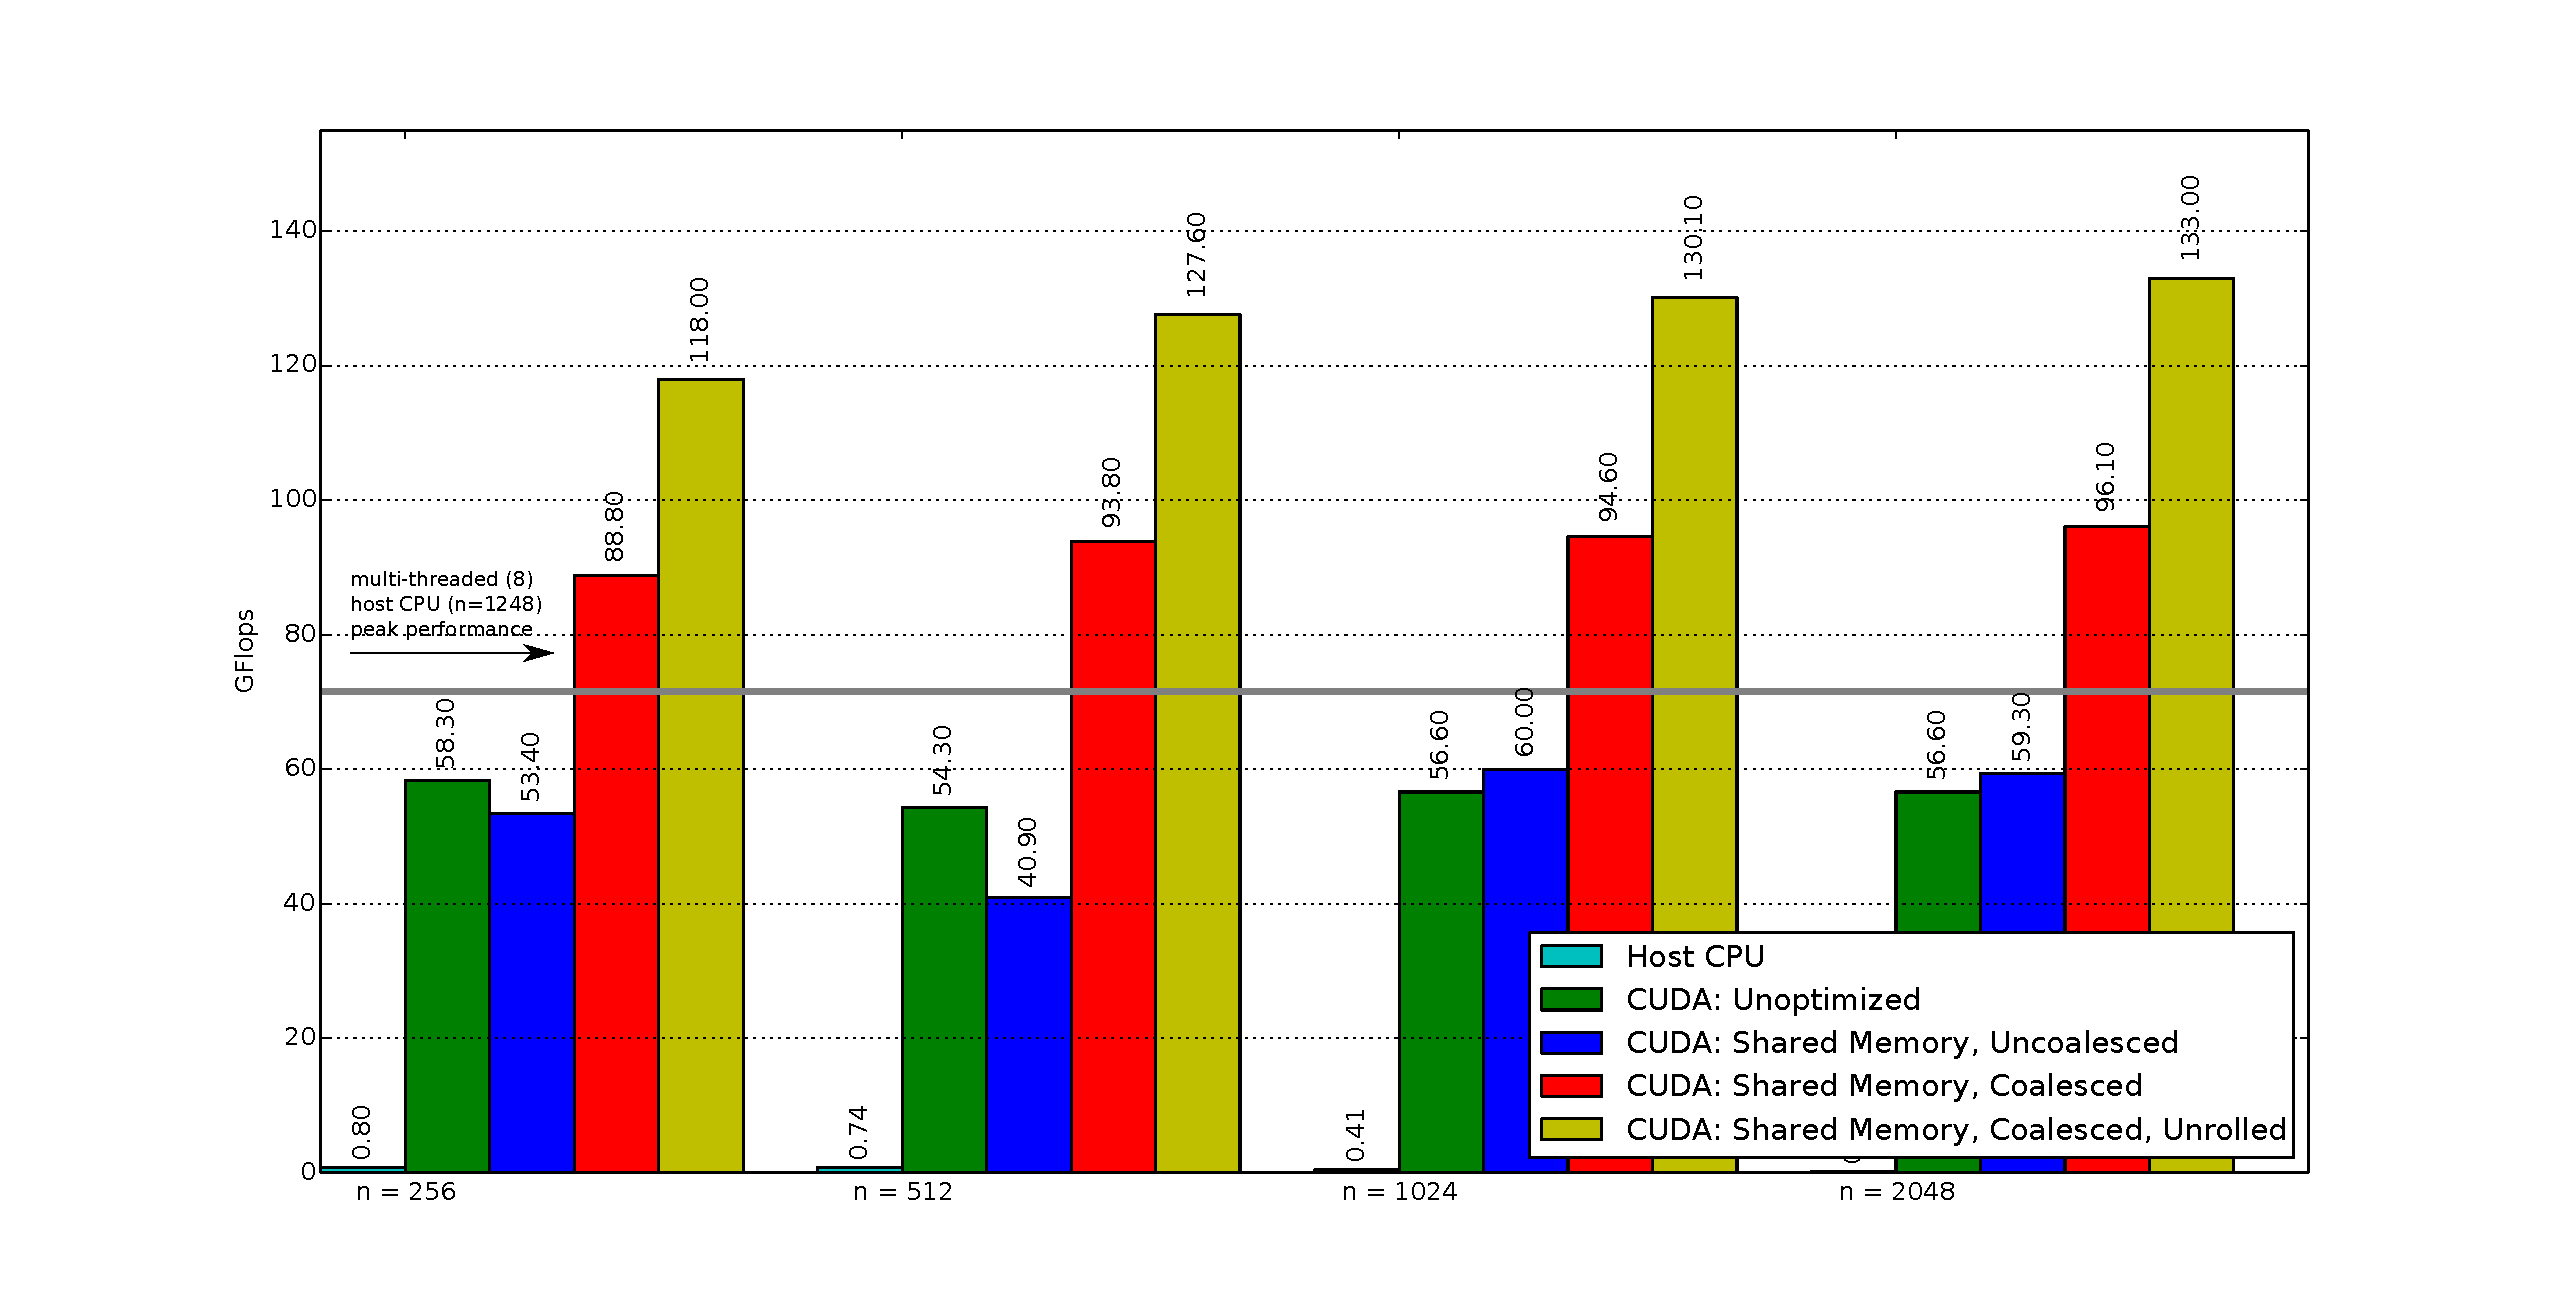
\includegraphics[width=\textwidth]{overview.pdf}
\caption{Performance Overview}
\label{fig:overview}
\end{figure}

For the unoptimized single-threaded host CPU computation, we reached the following performance.
\begin{itemize}
    \item $n=256$: 0.8 GFlops
    \item $n=512$: 0.74 GFlops
    \item $n=1024$: 0.41 GFlops
    \item $n=2048$: 0.15 GFlops
\end{itemize}

The performance of the multi-threaded optimized host CPU computation is shown in the previous section for various matrix sizes and number of threads.

\end{document}